\حصہ{نلکی چھلے}
اجسام طواف کا حجم تلاش کرتے ہوئے بعض اوقات چھلا کی بجائے نلکی خول استعمال کرنا زیادہ بہتر ثابت ہوتا ہے (شکل \حوالہ{شکل_تکمل_استعمال_جسم_طواف_نلکی_الف})۔
\begin{figure}
\centering
\begin{subfigure}{0.45\textwidth}
\centering
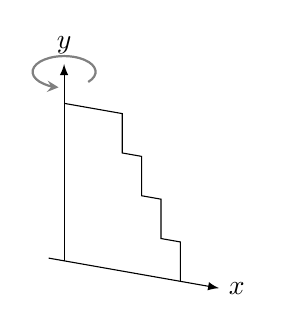
\begin{tikzpicture}[x={(-10:1)}]
\pgfmathsetmacro{\h}{0.5}
\pgfmathsetmacro{\hh}{0}
\pgfmathsetmacro{\ra}{1.5}
\pgfmathsetmacro{\dr}{0.25}
\draw[-latex](-0.2,0)--(2,0)node[right]{$x$};
\draw[-latex](0,0)--(0,2.5)node[above]{$y$};
\draw[thick,gray,-stealth] ([shift={(-40:0.4cm and 0.2cm)}]0,2.4) arc (-40:260:0.4cm and 0.2cm);
\draw(\ra,0)--++(0,\h)--++(-\dr,0)--++(0,\h)--++(-\dr,0)--++(0,\h)--++(-\dr,0)--++(0,\h)--++(-\ra+3*\dr,0);
\end{tikzpicture}
\caption{}
\end{subfigure}\hfill
\begin{subfigure}{0.45\textwidth}
\centering
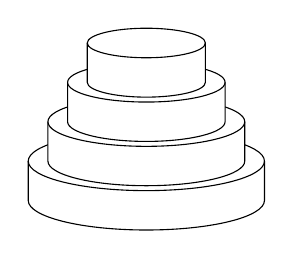
\begin{tikzpicture}[font=\small]
\pgfmathsetmacro{\h}{0.5}
\pgfmathsetmacro{\hh}{0}
\pgfmathsetmacro{\ra}{1.5}
\draw[fill=white]([shift={(0:\ra cm and 1/4*\ra cm)}]0,\hh) arc (0:180:\ra cm and 1/4*\ra cm)--++(0,-\h) arc (180:360:\ra cm and 1/4*\ra cm)--++(0,\h);
\draw([shift={(180:\ra cm and 1/4*\ra cm)}]0,\hh) arc (180:360:\ra cm and 1/4*\ra cm);
\pgfmathsetmacro{\hh}{\h}
\pgfmathsetmacro{\ra}{1.25}
\draw[fill=white]([shift={(0:\ra cm and 1/4*\ra cm)}]0,\hh) arc (0:180:\ra cm and 1/4*\ra cm)--++(0,-\h) arc (180:360:\ra cm and 1/4*\ra cm)--++(0,\h);
\draw([shift={(180:\ra cm and 1/4*\ra cm)}]0,\hh) arc (180:360:\ra cm and 1/4*\ra cm);
\pgfmathsetmacro{\hh}{2*\h}
\pgfmathsetmacro{\ra}{1}
\draw[fill=white]([shift={(0:\ra cm and 1/4*\ra cm)}]0,\hh) arc (0:180:\ra cm and 1/4*\ra cm)--++(0,-\h) arc (180:360:\ra cm and 1/4*\ra cm)--++(0,\h);
\draw([shift={(180:\ra cm and 1/4*\ra cm)}]0,\hh) arc (180:360:\ra cm and 1/4*\ra cm);
\pgfmathsetmacro{\hh}{3*\h}
\pgfmathsetmacro{\ra}{0.75}
\draw[fill=white]([shift={(0:\ra cm and 1/4*\ra cm)}]0,\hh) arc (0:180:\ra cm and 1/4*\ra cm)--++(0,-\h) arc (180:360:\ra cm and 1/4*\ra cm)--++(0,\h);
\draw([shift={(180:\ra cm and 1/4*\ra cm)}]0,\hh) arc (180:360:\ra cm and 1/4*\ra cm);
\end{tikzpicture}
\caption{}
\end{subfigure}
\caption{نلکی جسم طواف}
\label{شکل_تکمل_استعمال_جسم_طواف_نلکی_الف}
\end{figure}
\جزوحصہء{نلکی کلیہ}
فرض کریں ہم \عددی{x} محور اور   وقفہ \عددی{[a,b]} پر تفاعل \عددی{y=f(x)} کے بیچ خطے  کو \عددی{y} محور کے گرد گھما کر جسم طواف حاصل کرتے ہیں۔ہمیں جسم طواف کا حجم درکار ہے۔  ہم وقفہ \عددی{[a,b]} کی خانہ بندی \عددی{P} پر منحصر مستطیلوں کو خطے کا تخمینی رقبہ لے سکتے ہیں۔ ایک نمائندہ مستطیل کی چوڑائی \عددی{\Delta x_k} اور قد \عددی{f(c_k)} ہو گا، جہاں نمائندہ مستطیل کے قاعدے کا وسط \عددی{c_k} ہے (شکل \حوالہ{شکل_تکمل_استعمال_کے_ویں_مستطیل_کا_خول})۔ہم جیومیٹری سے جانتے ہیں کہ ایسے مستطیل کو \عددی{y} محور کے گرد گھمانے سے حاصل جسم طواف کا حجم
\begin{align*}
\Delta H_k=2\pi\times \text{\RL{خول کا اوسط رداس}}\times \text{\RL{خول کا قد}}\times \text{\RL{موٹائی}}
\end{align*}  
ہو گا جو موجودہ صورت میں درج ذیل ہو گا۔
\begin{align*}
\Delta H_k=2\pi c_k f(c_k)\Delta x_k
\end{align*}
ہم \عددی{P} پر منحصر \عددی{n} مستطیلوں کو \عددی{y} محور کے گرد گھمانے سے حاصل حجم کے مجموعہ کو تخمیناً جسم طواف کا حجم لیتے ہیں۔
\begin{align*} 
H\approx \sum_{k=1}^n\Delta H_k=\sum_{k=1}^n2\pi c_kf(c_k)\Delta x_k\quad\quad \text{\RL{ریمان مجموعہ}}
\end{align*}
\عددی{\norm{P}\to 0} کرتے ہوئے اس مجموعہ کا حد ٹھوس جسم کا حجم  ہو گا:
\begin{align*}
H=\lim_{\norm{P}\to 0}\sum_{k=1}^n2\pi c_kf(c_k)\Delta x_k=\int_a^b2\pi xf(x)\dif x
\end{align*}
%
\begin{figure}
\centering
\begin{tikzpicture}[font=\small,declare function={f(\x)=2-sqrt(\x);}]
\pgfmathsetmacro{\c}{1.5}
\pgfmathsetmacro{\w}{0.2}
\pgfmathsetmacro{\ra}{\c-\w}
\pgfmathsetmacro{\rb}{\c+\w}
\pgfmathsetmacro{\angS}{0}
\pgfmathsetmacro{\angE}{240}
\pgfmathsetmacro{\d}{0.5}
\draw[-latex](0,0)--++(2.5,0)node[right]{$x$};
\draw[-latex](0,0)--++(0,2.5)node[above]{$y$};
\draw[thick,gray,-stealth]([shift={(-20:0.4cm and 0.2cm)}]0,2) arc (-20:240:0.4cm and 0.2cm);
\draw[thick]plot[domain=0.2:2]({\x},{f(\x)});
\draw[thick](0.2,0)--++(0,{f(0.2)})  (2,0)--++(0,{f(2)});
\draw(\d,{f(\d)})--++(45:0.5)node[right]{$y=f(x)$};
\draw([shift={(\angS:\ra cm and 1/4*\ra cm)}]0,{f(\c)}) arc (\angS:\angE:\ra cm and 1/4*\ra cm);
\draw([shift={(\angS:\rb cm and 1/4*\rb cm)}]0,{f(\c)}) arc (\angS:\angE:\rb cm and 1/4*\rb cm);
\draw([shift={(\angS:\ra cm and 1/4*\ra cm)}]0,0) arc (\angS:\angE:\ra cm and 1/4*\ra cm);
\draw(\ra,{f(\c)})coordinate(sI)--(\rb,{f(\c)})coordinate(sO);
\draw(sI)--++(0,-{f(\c)})  (sO)--++(0,{-f(\c)});
\path(0,{f(\c)})++(\angE:\ra cm and 1/4*\ra cm)coordinate(eI)++(0,{-f(\c)})coordinate(eIL);
\path(0,{f(\c)})++(\angE:\rb cm and 1/4*\rb cm)coordinate(eO)++(0,{-f(\c)})coordinate(eOL);
\fill[white](eO)--(eOL)--++(-1/2*\ra,0)--++(0,{f(\c)})--cycle;
\draw[fill=white](eI)--(eO)--(eOL)--(eIL)--(eI);
\draw([shift={(180:\rb cm and 1/4*\rb cm)}]0,0) arc (180:\angE:\rb cm and 1/4*\rb cm);
\draw(-\rb,0)--++(0,{f(\c)});
\draw(\c,0)node[below]{$c_k$}--++(0,0.1);
\draw(\c-\w,-0.4)--++(0,-0.3)coordinate[pos=0.5](kL);
\draw(\c+\w,-0.4)--++(0,-0.3)coordinate[pos=0.5](kR);
\draw[stealth-](kL)--++(-0.2,0);
\draw[stealth-](kR)--++(0.2,0)--++(0,-0.3)node[below]{$\Delta x_k$};
\draw(\c+\w,0)++(0,-0.1)--++(-55:0.7)--++(0.2,0)node[right]{$x_k$}  (\c-\w,0)++(0,-0.1)--++(-135:0.7)node[left]{$x_{k-1}$};
\draw[fill=lgray,opacity=0.5](\c-\w,0)--++(0,{f(\c)})--++(2*\w,0)--++(0,{-f(\c)})--cycle;
\draw[stealth-stealth](2.2,0)--++(0,{f(\c)})node[pos=0.75,right]{\text{\RL{قد مستطیل}}};
\draw(2.1,{f(\c)})--++(0.2,0);
\draw(0.2,0)node[below]{$a$}--++(0,0.1);
\draw(2,0)node[below]{$b$}--++(0,0.1);
\end{tikzpicture}
\caption{$k$ ویں مستطیل کو گھمانے سے حاصل نلکی خول۔}
\label{شکل_تکمل_استعمال_کے_ویں_مستطیل_کا_خول}
\end{figure}

\موٹا{کلیہ خول برائے $y$ محور کے گرد طواف}\\
استمراری تفاعل \عددی{y=f(x),\, 0\le a\le x\le b} اور محور \عددی{x} کے بیچ خطے کو \عددی{y} محور کے گرد گھمانے سے حاصل جسم طواف کا حجم درج ذیل ہو گا۔
\begin{align}\label{مساوات_تکمل_استعمال_کلیہ_خول_وائے_محور}
H=\int_a^b2\pi(\text{\RL{رداس خول}})(\text{\RL{قد خول}})\dif x=\int_a^b2\pi xf(x)\dif x
\end{align}

\ابتدا{مثال}\شناخت{مثال_تکمل_استعمال_نلکی_پہلی}
منحنی \عددی{y=\sqrt{x}}، لکیر \عددی{x=4} اور \عددی{x} محور کے بیچ خطے کو \عددی{y} محور کے گرد گھما کر جسم طواف حاصل کیا جاتا ہے۔ اس جسم کا حجم تلاش کریں۔
\begin{figure}
\centering
\begin{subfigure}{0.30\textwidth}
\centering
\begin{tikzpicture}[font=\small,declare function={f(\x)=sqrt(\x);}]
\pgfmathsetmacro{\c}{1.7}
\draw[-latex](-0.25,0)--(4.25,0)node[right]{$x$};
\draw[-latex](0,-0.2)--(0,2.6)node[above]{$y$};
\draw[gray,thick,-stealth]([shift={(-20:0.4cm and 0.2cm)}]0,2.45) arc (-20:240:0.4cm and 0.2cm);
\draw[]plot[domain=0:0.5]({\x},{f(\x)});
\draw[]plot[domain=0.5:4]({\x},{f(\x)});
\draw[](4,0)node[below]{$4$}--(4,{f(4)})node[above left,yshift=-1ex]{$y=\sqrt{x}$};
\draw(0,2)node[left]{$2$}--++(0.1,0);
\draw[thick](\c,0)node[circ]{}node[below]{$x$}--++(0,{f(\c)})node[circ]{}coordinate(kT);
\draw[stealth-stealth] (\c+0.4,0)--++(0,{f(\c)})node[pos=0.5,right]{$f(x)=\sqrt{x}$}coordinate[pos=0.5](kH);
\draw(\c+0.3,{f(\c)})--++(0.2,0);
\draw[stealth-stealth](\c,{f(\c)+0.2})--++(-\c,0)node[pos=0.5,fill=white]{$x$}coordinate[pos=0.5](kR);
\draw(\c,{f(\c)+0.1})--++(0,0.2);
\draw(kR)node[above]{\RL{رداس خول}};
\draw(kH)++(0.3,0.2)node[above right]{\RL{قد خول}};
\draw(kT)++(0.1,0.1)--++(60:1.25)node[above]{\text{\RL{$\dif x$= موٹائی خول}}};
\draw [decorate,decoration={brace,amplitude=10pt,mirror,raise=4pt},yshift=0pt]
(0,-0.3) -- (4,-0.3) node [black,midway,yshift=-0.8cm] {\footnotesize \RL{وقفہ تکمل}};
\end{tikzpicture}
\caption{}
\end{subfigure}\hfill
\begin{subfigure}{0.60\textwidth}
\centering
\begin{tikzpicture}[font=\small,declare function={f(\x)=sqrt(\x);}]
\pgfmathsetmacro{\c}{1.7}
\pgfmathsetmacro{\w}{0.2}
\pgfmathsetmacro{\ra}{\c-\w}
\pgfmathsetmacro{\rb}{\c+\w}
\pgfmathsetmacro{\hy}{f(\c)-1/4*\ra}
\draw[dashed](-0.25,0)--(\rb,0);
\draw[-latex](\rb,0)--(4.25,0)node[right]{$x$};
\draw[dashed](0,-0.2)--(0,\hy);
\draw[-latex](0,\hy)--(0,2.6)node[above]{$y$};
\draw[dashed]plot[domain=0:0.5]({\x},{f(\x)});
\draw[dashed]plot[domain=0.5:\rb]({\x},{f(\x)});
\draw[]plot[domain=\rb:4]({\x},{f(\x)});
\draw(4,{f(4)})node[above left]{$y=\sqrt{x}$};
\draw(0,{f(\c)}) circle (\ra cm and 1/4*\ra cm);
\draw(0,{f(\c)}) circle (\rb cm and 1/4*\rb cm);
\draw([shift={(180:\rb cm and 1/4*\rb cm)}]0,0)arc (180:360:\rb cm and 1/4*\rb cm);
\draw(\rb,0)--(\rb,{f(\c)})  (-\rb,0)--(-\rb,{f(\c)});
\draw[thick,gray](\c,0)node[circ]{}node[above left,black]{$x$}--(\c,{f(\c)})node[circ]{};
\draw(4,0)node[below]{$4$}--++(0,0.1);
\draw[stealth-stealth](\rb+0.3,{f(\c)})--(\rb+0.3,0)node[pos=0.5,right]{$\sqrt{x}$};
\draw(\rb+0.2,{f(\c)})--++(0.2,0);
\draw[stealth-](\ra,-0.5)--++(-0.2,0);
\draw[stealth-](\rb,-0.5)--++(0.2,0)node[right]{$\dif x$};
\draw(\ra,-0.4)--++(0,-0.2)  (\rb,-0.4)--++(0,-0.2);
\end{tikzpicture}
\caption{}
\end{subfigure}
\caption{نلکی خول (مثال \حوالہ{مثال_تکمل_استعمال_نلکی_پہلی})}
\label{شکل_مثال_تکمل_استعمال_نلکی_پہلی}
\end{figure}

حل:\quad
\موٹا{پہلا قدم:}\quad
خطے کا خاکہ بنا کر محور گردش کے متوازی اس پر قطع دکھائیں۔ قطع کا قد (خول کا قد) اور محور گردش سے قطع کے فاصلہ (رداس خول) کی نشاندہی کریں۔ قطع کی چوڑائی \عددی{\dif x} خول کی چوڑائی ہو گی۔ ہم نے شکل \حوالہ{شکل_مثال_تکمل_استعمال_نلکی_پہلی} میں خول دکھایا ہے۔ آپ کو ایسا کرنے کی ضرورت نہیں ہے۔\\
\موٹا{دوسرا قدم:}\quad
تکمل کے حد معلوم کریں۔ خطہ میں \عددی{x} کی قیمت \عددی{a} تا \عددی{b} تبدیل ہوتی ہے لہٰذا تکمل کے حد \عددی{a} اور \عددی{b} ہوں گے۔
\begin{align*}
H&=\int_a^b2\pi(\text{\RL{رداس خول}})(\text{\RL{قد خول}})\dif x
&&\text{\RL{مساوات \حوالہ{مساوات_تکمل_استعمال_کلیہ_خول_وائے_محور}}}\\
&=\int_0^4 2\pi(x)(\sqrt{x})\dif x&&\text{\RL{جزو-ا اور جزو-ب میں حاصل قیمتیں}}\\
&=2\pi\int_0^4x^{3/2}\dif x=2\pi\big[\frac{2}{5}x^{5/2}\big]_0^4=\frac{128\pi}{5}
\end{align*} 
\انتہا{مثال}
%=====================
محور \عددی{y} کے گرد خطہ گھمانے سے حاصل جسم طواف کا حجم مساوات \حوالہ{مساوات_تکمل_استعمال_کلیہ_خول_وائے_محور} سے حاصل کیا جا سکتا ہے۔اگر ہم خطے کو \عددی{x} محور کے گرد گھما کر جسم طواف حاصل کریں تب حجم تلاش کرنے کی خاطر مساوات \حوالہ{مساوات_تکمل_استعمال_کلیہ_خول_وائے_محور} میں \عددی{x} کی جگہ \عددی{y} استعمال کیا جائے گا۔

\موٹا{کلیہ خول برائے $x$ محور کے گرد طواف}\\
\begin{align}\label{مساوات_تکمل_استعمال_کلیہ_خول_ایکس_محور}
H=\int_c^d2\pi(\text{\RL{رداس خول}})(\text{\RL{قد خول}})\dif y=\int_c^d2\pi yf(y)\dif y
\end{align}
درج بالا مساوات میں \عددی{f(y)>0} اور \عددی{0\le c\le y\le d} ہیں۔ 

\ابتدا{مثال}\شناخت{مثال_تکمل_استعمال_پہلے_بھی-حل}
منحنی \عددی{y=\sqrt{x}}، لکیر \عددی{x=4} اور \عددی{x} محور کے بیچ خطے کو \عددی{x} محور کے گرد گھما کر جسم طواف حاصل کیا جاتا ہے۔ اس جسم کا حجم تلاش کریں۔

حل:\quad
\موٹا{پہلا قدم:}\quad
خطے کا خاکہ بنائیں اور اس پر محور گردش کے متوازی قطع دکھائیں۔ قطع کی لمبائی (قد خول) اور محور طواف سے اس کا فاصلہ (رداس خول) کی نشاندہی کریں۔ قطع کی موٹائی، خول کی چوڑائی \عددی{\dif y} ہو گی۔ ہم نے شکل \حوالہ{شکل_مثال_تکمل_استعمال_پہلے_بھی-حل} میں \عددی{y} محور کے گرد بیلن دکھایا ہے۔ آپ کو ایسا بنانے کی ضرورت نہیں ہے۔\\
\موٹا{دوسرا قدم:}\quad
تکمل کے حد معلوم کریں۔چونکہ خطہ میں \عددی{y} کی قیمت \عددی{c=0} تا \عددی{d=2} ہو سکتی ہے لہٰذا یہی اس کے حد ہیں۔\\
\موٹا{تیسرا قدم:}\quad
\begin{align*}
H&=\int_c^d2\pi(رداس خول)(قد خول)\dif y&&\text{\RL{مساوات \حوالہ{مساوات_تکمل_استعمال_کلیہ_خول_ایکس_محور}}}\\
&=\int_0^22\pi(y)(4-y^2)\dif y&&\text{\RL{جزو-ا اور جزو-ب میں حاصل قیمتیں}}\\
&=2\pi\big[2y^2-\frac{y^4}{4}\big]_0^2=8\pi
\end{align*}
یہ نتیجہ مثال \حوالہ{مثال_تکمل_استعمال_جسم_طواف_جذر} میں  ترکیب قرص سے حاصل جواب کے عین مطابق ہے۔ 
\انتہا{مثال}
%====================
\begin{figure}
\centering
\begin{subfigure}{0.45\textwidth}
\centering
\begin{tikzpicture}[font=\small,declare function={f(\x)=sqrt(\x);}]
\pgfmathsetmacro{\c}{1.25}
\draw[-latex](-0.25,0)--(4.5,0)node[right]{$x$};
\draw[-latex](0,-0.2)--(0,2.25)node[above]{$y$};
\draw[gray,thick,-stealth] ([shift={(-100:0.2cm and 0.4cm)}]4.4,0) arc (-100:160:0.2cm and 0.4cm);
\draw[]plot[domain=0:0.5]({\x},{f(\x)});
\draw[]plot[domain=0.5:4]({\x},{f(\x)});
\draw(4,0)node[below]{$4$}--(4,2);
\draw(4,{f(4)})node[above left]{$y=\sqrt{x}$};
\draw[thick](\c,{f(\c)})node[circ]{}--(4,{f(\c)})node[circ]{}node[pos=0.6,above]{\RL{قد خول}}node[pos=0.6,below]{$4-y^2$};
\draw[stealth-stealth](\c-0.3,0)--++(0,{f(\c)})node[pos=0.5,left]{$y$}node[pos=0.5,right]{\RL{رداس خول}};
\draw(\c-0.2,{f(\c)})--++(-0.2,0);
\draw[stealth-](4.2,{f(\c)})++(0,0.01)--++(0,0.2)--++(0.2,0)node[right]{$\dif y$};
\draw[stealth-](4.2,{f(\c)})++(0,-0.01)--++(0,-0.2);
\draw(0,2)node[left]{$2$}--++(0.1,0);
\draw(0,{f(\c)})node[left]{$y$}--++(0.1,0);
\draw [decorate,decoration={brace,amplitude=10pt,mirror},yshift=0pt]
(-0.4,2) -- (-0.4,0) node [black,midway,xshift=-0.8cm] {\footnotesize \RL{وقفہ تکمل}};
\end{tikzpicture}
\caption{}
\end{subfigure}\hfill
\begin{subfigure}{0.45\textwidth}
\centering
\begin{tikzpicture}[font=\small,declare function={f(\x)=sqrt(\x);}]
\pgfmathsetmacro{\c}{1.25}
\pgfmathsetmacro{\w}{0.2}
\pgfmathsetmacro{\ra}{f(\c)+\w}
\pgfmathsetmacro{\rb}{f(\c)-\w}
\pgfmathsetmacro{\xx}{(\w+f(\c))^2}
\draw(-0.25,0)--(\c+1/4*\ra,0);
\draw[dashed](\c+1/4*\rb,0)--(4+1/4*\rb,0);
\draw[-latex](4+1/4*\ra,0)--(5,0)node[right]{$x$};
\draw[-latex](0,-0.2)--(0,2.5)node[above]{$y$};
\draw[]plot[domain=0:0.5]({\x},{f(\x)});
\draw[]plot[domain=0.5:\c]({\x},{f(\x)});
\draw[dashed]plot[domain=\c:\xx]({\x},{f(\x)});
\draw[]plot[domain=\xx:4]({\x},{f(\x)});
\draw(4,{f(4)})--(4,{f(\c)+\w});
\draw(2.5,{f(2.5)})node[left,yshift=1ex]{$y=\sqrt{x}$};
\draw[dashed](4,{f(\c)+\w})--(4,0)node[below]{$4$};
\draw[stealth-stealth](\c,0)--(\c,{f(\c)})node[pos=0.45,fill=white]{$y$};
\draw(\c,0) circle (1/4*\ra cm and \ra cm);
\draw(\c,0) circle (1/4*\rb cm and \rb cm);
\draw([shift={(-90:1/4*\ra cm and \ra cm)}]4,0) arc (-90:90:1/4*\ra cm and \ra cm);
\draw[dashed]([shift={(90:1/4*\ra cm and \ra cm)}]4,0) arc (90:270:1/4*\ra cm and \ra cm);
\draw[dashed]([shift={(0:1/4*\rb cm and \rb cm)}]4,0) arc (0:360:1/4*\rb cm and \rb cm);
\draw(\c,{f(\c)+\w})--(4,{f(\c)+\w})   (\c,{-f(\c)-\w})--(4,{-f(\c)-\w});
\draw[gray,thick](\c,{f(\c)})node[circ]{}--(4,{f(\c)})node[circ]{};
\draw[stealth-stealth](\c,2.2)--(4,2.2)node[pos=0.5,above]{$4-y^2$};
\draw(\c,2.1)--++(0,0.2)  (4,2.1)--++(0,0.2);
\draw(4.3,{f(\c)+\w})--++(0.2,0)coordinate[pos=0.5](kt);
\draw(4.3,{f(\c)-\w})--++(0.2,0)coordinate[pos=0.5](kb);
\draw[stealth-](kb)--++(0,-0.2);
\draw[stealth-](kt)--++(0,0.2)--++(0.2,0)node[right]{$\dif y$};
\end{tikzpicture}
\caption{}
\end{subfigure}
\caption{محور \عددی{} کے گرد طواف (مثال \حوالہ{مثال_تکمل_استعمال_پہلے_بھی-حل})}
\label{شکل_مثال_تکمل_استعمال_پہلے_بھی-حل}
\end{figure}

\جزوحصہء{ترکیب خول کا استعمال}
محور طواف (افقی یا انتصابی) جیسا بھی ہو ترکیب خول کے اقدام درج ذیل ہوں گے۔
\begin{enumerate}[a.]
\item
خطے کا خاکہ بنا کر اس میں محور طواف کے متوازی قطع بنائیں۔ قطع کا قد یا لمبائی (قد خول)،  محور طواف سے قطع کا فاصلہ (رداس خول) اور قطع کی موٹائی (چوڑائی خول) کی نشاندہی کریں۔
\item
تکمل کے حد معلوم کریں
\item
متکمل (\عددی{2\pi}) ( رداس خول ) ( قد خول )  کا موزوں متغیر (\عددی{x} یا \عددی{y}) کے ساتھ تکمل کی قیمت حاصل کرتے ہوئے حجم دریافت کریں۔
\end{enumerate} 

اگلی مثال میں محور طواف افقی لکیر \عددی{x=2} ہے۔

\ابتدا{مثال}\شناخت{مثال_تکمل_استعمال_خول_آخری}
ربع اول میں قطع مکافی \عددی{y=x^2}، لکیر \عددی{y=1} اور \عددی{y} محور کے بیچ خطے کو محور طواف \عددی{x=2} کے گرد گھما کر جسم طواف پیدا کیا جاتا ہے۔اس جسم کا حجم تلاش کریں۔

حل:\quad
\موٹا{پہلا قدم:}\quad
خطے پر محور طواف کے متوازی قطع بنائیں۔ قطع کا قد (قد خول)، محور طواف سے قطع کا فاصلہ (رداس خول) اور قطع کی موٹائی (چوڑائی خول \عددی{\dif x}) کی نشاندہی کریں (شکل \حوالہ{شکل_مثال_تکمل_استعمال_خول_آخری})۔ہم نے خول بھی بنایا ہے۔ آپ کو ایسا کرنے کی ضرورت نہیں ہے۔\\
\موٹا{دوسرا قدم:}\quad
تکمل کے حد \عددی{a=0} اور \عددی{b=1} ہیں۔\\
\موٹا{تیسرا قدم:}
\begin{align*}
H&=\int_a^b2\pi(\text{\RL{رداس خول}})(\text{\RL{قد خول}})\dif x&&\text{\RL{مساوات \حوالہ{مساوات_تکمل_استعمال_کلیہ_خول_وائے_محور}}}\\
&=\int_0^12\pi(2-x)(1-x^2)\dif x&&\text{\RL{جزو-ا اور جزو-ب میں حاصل قیمتیں}}\\
&=2\pi\int_0^1(2-x-2x^2+x^3)\dif x\\
&=\frac{13\pi}{6}
\end{align*}
\انتہا{مثال}
%=======================
\begin{figure}
\centering
\begin{subfigure}{0.45\textwidth}
\centering
\begin{tikzpicture}[scale=2,font=\small,declare function={f(\x)=\x^2;}]
\pgfmathsetmacro{\c}{0.7}
\draw[-latex](-0.25,0)--(2.25,0)node[right]{$x$};
\draw[-latex](0,-0.2)--(0,1.25)node[above]{$y$};
\draw[]plot[domain=0:1]({\x},{f(\x)});
\draw(0.6,{f(0.6)})node[left]{$y=x^2$};
\draw(1,{f(1)})--(0,{f(1)})node[left]{$1$}node[pos=0.6,above]{$y=1$};
\draw(\c,{f(\c)})node[circ]{}--(\c,1)node[circ]{};
\draw(\c,0)node[below]{$x$}--++(0,0.1);
\draw(1,0)node[below]{$1$}--++(0,0.1);
\draw [decorate,decoration={brace,amplitude=10pt,mirror,raise=4pt},yshift=0pt]
(0,-0.2) -- (1,-0.2) node [black,midway,yshift=-0.8cm] {\footnotesize \RL{وقفہ تکمل}};
\draw(2,0)node[below]{$2$}--(2,1.25);
\draw[gray,thick,-stealth]([shift={(-40:0.2cm and 0.1cm)}]2,1.2) arc (-40:240:0.2cm and 0.1cm);
\draw[stealth-stealth](1.2,{f(\c)})--(1.2,1)node[pos=0.7,right]{\text{\RL{قد خول}}} node[pos=0.4,right]{$1-x^2$};
\draw(1.1,{f(\c)})--++(0.2,0)   (1.1,1)--++(0.2,0);
\draw(\c,1)++(0,0.1)--++(45:0.25)node[above]{\text{\RL{موٹائی خول=$\dif x$}}};
\draw[stealth-stealth](\c,{f(\c)-0.2})--(2,{f(\c)-0.2})node[pos=0.7,yshift=1ex]{$2-x$}node[pos=0.7,yshift=-1.25ex]{\text{\RL{رداس خول}}};
\draw(\c,{f(\c)-0.15})--++(0,-0.1);
\end{tikzpicture}
\caption{}
\end{subfigure}\hfill
\begin{subfigure}{0.45\textwidth}
\centering
\begin{tikzpicture}[font=\small,declare function={f(\x)=\x^2;}]
\pgfmathsetmacro{\c}{0.7}
\pgfmathsetmacro{\w}{0.1}
\pgfmathsetmacro{\ra}{2-\c+\w}
\pgfmathsetmacro{\rb}{2-\c-\w}
\draw[-latex](-0.25,0)--(4,0)node[right]{$x$};
\draw[-latex](0,-0.2)--(0,1.5)node[above]{$y$};
\draw[]plot[domain=0:1]({\x},{f(\x)});
\draw(1,{f(1)})--(0,{f(1)});
\draw(\c,{f(\c)})node[circ]{}--(\c,1)node[circ]{};
\draw(2,1) circle (\ra cm and 1/4*\ra cm);
\draw(2,1) circle (\rb cm and 1/4*\rb cm);
\draw([shift={(180:\ra cm and 1/4*\ra cm)}]2,{f(\c)}) arc (180:360:\ra cm and 1/4*\ra cm);
\draw(\c-\w,{f(\c)})--(\c-\w,1)  (2+\ra,{f(\c)})--(2+\ra,1);
\draw(2,{f(\c)-1/4*\ra})--(2,0)node[below]{$2$};
\draw(2,{1-1/4*\rb})--++(0,1);
\draw[stealth-stealth](\c,1.5)--(2,1.5)node[pos=0.5,above]{$1-x^2$};
\draw(\c,1.3)--++(0,0.3);
\draw[stealth-stealth](2+\ra+0.3,{f(\c)})--(2+\ra+0.3,1)node[pos=0.5,right]{$1-x^2$};
\draw(2+\ra+0.2,{f(\c)})--++(0.2,0)  (2+\ra+0.2,1)--++(0.2,0);
\draw[stealth-](2+\rb,1.5)--++(-0.3,0);
\draw[stealth-](2+\ra,1.5)--++(0.3,0)node[right]{$\dif x$};
\draw(2+\rb,1.4)--++(0,0.2) (2+\ra,1.4)--++(0,0.2);
\end{tikzpicture}
\caption{}
\end{subfigure}\hfill
\caption{خطہ اور خول (مثال \حوالہ{مثال_تکمل_استعمال_خول_آخری})}
\label{شکل_مثال_تکمل_استعمال_خول_آخری}
\end{figure}
%
\begin{figure}
\centering
\begin{subfigure}{0.45\textwidth}
\begin{tikzpicture}[scale=2,font=\small,declare function={f(\x)=\x^2;g(\x)=\x;}]
\pgfmathsetmacro{\c}{0.4}
\pgfmathsetmacro{\ra}{\c}
\pgfmathsetmacro{\rb}{sqrt(\c)}
\draw[gray,thick,-stealth]([shift={(-40:0.2cm and 0.1cm)}]0,1.2) arc (-40:240:0.2cm and 0.1cm);
\draw[]plot[domain=0:1]({\x},{f(\x)});
\draw[]plot[domain=0:1]({\x},{g(\x)});
\draw(1,0)node[below]{$1$}--++(0,0.1);
\draw(0,1)node[left]{$1$}--++(0.1,0);
\draw(0.8,{g(0.8)})node[left]{$x=y$};
\draw(0.8,{f(0.8)})node[right]{$x=\sqrt{y}$};
\draw[thick](\ra,\c)node[circ]{}--(\rb,\c)node[circ]{};
\draw[fill=lgray,opacity=0.5](0,\c) circle (\rb cm and 1/4*\rb cm);
\draw[fill=white](0,\c) circle (\ra cm and 1/4*\ra cm);
\draw[-latex](-0.25,0)--(1.25,0)node[right]{$x$};
\draw(0,-0.5)--(0,\c-1/4*\rb);
\draw[-latex](0,\c-1/4*\ra)--(0,1.25)node[above]{$y$};
\draw[stealth-stealth](0,-0.3)--++(\ra,0)node[pos=0.5,above]{$r=y$};
\draw[stealth-stealth](0,-0.5)--++(\rb,0)node[pos=0.5,below]{$R=\sqrt{y}$};
\draw(\ra,-0.2)--++(0,-0.2)  (\rb,-0.4)--++(0,-0.2);
\draw(0.5,-1)node[font=\footnotesize]{$\begin{aligned}H&=\int_{y=0}^{y=1}\pi[(\sqrt{y})^2-(y)^2]\dif y=\tfrac{\pi}{6}  \end{aligned}$};
\end{tikzpicture}
\caption{}
\end{subfigure}\hfill
\begin{subfigure}{0.45\textwidth}
\begin{tikzpicture}[scale=2,font=\small,declare function={f(\x)=\x^2;g(\x)=\x;}]
\pgfmathsetmacro{\c}{0.6}
\draw[gray,thick,-stealth]([shift={(-40:0.2cm and 0.1cm)}]0,1.2) arc (-40:240:0.2cm and 0.1cm);
\draw[]plot[domain=0:1]({\x},{f(\x)});
\draw[]plot[domain=0:1]({\x},{g(\x)});
\draw(1,0)node[below]{$1$}--++(0,0.1);
\draw(0,1)node[left]{$1$}--++(0.1,0);
\draw(0.9,{g(0.9)})node[left]{$y=x$};
\draw(0.9,{f(0.9)})node[right,xshift=1ex]{$y=x^2$};
\draw[thick](\c,{f(\c)})node[circ]{}--(\c,\c)node[circ]{};
\draw[-latex](-0.25,0)--(1.25,0)node[right]{$x$};
\draw[-latex](0,-0.5)--(0,1.25)node[above]{$y$};
\draw[fill=lgray,opacity=0.5]([shift={(180:\c cm and 1/4*\c cm)}]0,{f(\c)}) arc (180:360:\c cm and 1/4*\c cm)--(\c,\c) arc (0:-180:\c cm and 1/4*\c cm)--(-\c,{f(\c)});
\draw([shift={(0:\c cm and 1/4*\c cm)}]0,\c) arc (0:180:\c cm and 1/4*\c cm);
\draw[stealth-stealth](\c+0.1,0)--(\c+0.1,{f(\c)})node[pos=0.4,left]{$x^2$};
\draw(\c+0.05,{f(\c)})--+(0.1,0);
\draw[stealth-stealth](\c+0.3,0)--(\c+0.3,{g(\c)})node[pos=0.5,right]{$x$};
\draw(\c+0.25,{g(\c)})--+(0.1,0);
\draw[stealth-stealth](0,{g(\c)})--(\c,{g(\c)})node[pos=0.5,fill=white]{$x$};
\draw(0.5,-1)node[font=\footnotesize]{$\begin{aligned}H&=\int_{x=0}^{x=1}2\pi(x)(x-x^2)\dif x=\frac{\pi}{6} \end{aligned}$};
\end{tikzpicture}
\caption{}
\end{subfigure}
\begin{subfigure}{0.45\textwidth}
\begin{tikzpicture}[scale=2,font=\small,declare function={f(\x)=\x^2;g(\x)=\x;}]
\pgfmathsetmacro{\c}{0.6}
\pgfmathsetmacro{\ra}{f(\c)}
\pgfmathsetmacro{\rb}{g(\c)}
\draw[gray,thick,-stealth]([shift={(-40:0.05cm and 0.15cm)}]1.2,0) arc (-40:240:0.05cm and 0.15cm);
\draw[]plot[domain=0:1]({\x},{f(\x)});
\draw[]plot[domain=0:1]({\x},{g(\x)});
\draw(1,0)node[below]{$1$}--++(0,0.1);
\draw(0,1)node[left]{$1$}--++(0.1,0);
\draw(0.9,{g(0.9)})node[left]{$y=x$};
\draw(0.9,{f(0.9)})node[right]{$y=x^2$};
\draw[fill=lgray,opacity=0.5](\c,0) circle (1/4*\rb cm and \rb cm);
\draw[fill=white](\c,0) circle (1/4*\ra cm and \ra cm);
\draw(-0.25,0)--(\c-1/4*\rb,0);
\draw[-latex](\c-1/4*\ra,0)--(1.25,0)node[right]{$x$};
\draw[-latex](0,-0.5)--(0,1.25)node[above]{$y$};
\draw(\c,{f(\c)})node[circ]{}--(\c,{g(\c)})node[circ]{};
\draw[stealth-stealth](\c+0.2,0)--++(0,{f(\c)})node[pos=0.8,right]{$r=x^2$};
\draw(\c+0.15,{f(\c)})--++(0.1,0);
\draw[stealth-stealth](-0.2,0)--++(0,{g(\c)})node[pos=0.5,left]{$R=x$};
\draw(-0.25,{g(\c)})--++(0.1,0);
\draw(0.5,-1)node[font=\footnotesize]{$\begin{aligned}H&=\int_{x=0}^{x=1}\pi[(x)^2-(x^2)^2]\dif x=\tfrac{2\pi}{15}  \end{aligned}$};
\end{tikzpicture}
\caption{}
\end{subfigure}\hfill
\begin{subfigure}{0.45\textwidth}
\begin{tikzpicture}[scale=2,font=\small,declare function={f(\x)=\x^2;g(\x)=\x;}]
\pgfmathsetmacro{\c}{0.4}
\pgfmathsetmacro{\ra}{\c}
\pgfmathsetmacro{\rb}{sqrt(\c)}
\draw[gray,thick,-stealth]([shift={(-40:0.05cm and 0.15cm)}]1.2,0) arc (-40:240:0.05cm and 0.15cm);
\draw[]plot[domain=0:1]({\x},{f(\x)});
\draw[]plot[domain=0:1]({\x},{g(\x)});
\draw(1,0)node[below]{$1$}--++(0,0.1);
\draw(0,1)node[left]{$1$}--++(0.1,0);
\draw(0.9,{g(0.9)})node[left]{$x=y$};
\draw(0.9,{f(0.9)})node[right]{$x=\sqrt{y}$};
\draw(\ra,\c)node[circ]{}--(\rb,\c)node[circ]{};
\draw[fill=lgray,opacity=0.5](\rb,\c)--(\ra,\c) arc (90:270:1/4*\c cm and \c cm)--(\rb,-\c) arc (-90:-270:1/4*\c cm and \c cm);
\draw([shift={(-90:1/4*\c cm and \c cm)}]\rb,0) arc (-90:90:1/4*\c cm and \c cm);
\draw[stealth-stealth](0,\c+0.1)--++(\c,0)node[pos=0.5,above]{$y$};
\draw(\c,\c+0.05)--++(0,0.1);
\draw[stealth-stealth](0,-\c-0.1)--++(\rb,0)node[pos=0.5,below]{$\sqrt{y}$};
\draw(\rb,-\c-0.05)--++(0,-0.1);
\draw(-0.25,0)--(\c-1/4*\c,0);
\draw[-latex](\rb-1/4*\c,0)--(1.25,0)node[right]{$x$};
\draw[-latex](0,-0.6)--(0,1.25)node[above]{$y$};
\draw(0,\c)node[left]{$y$}--++(0.1,0);
\draw(0.5,-1)node[font=\footnotesize]{$\begin{aligned}H&=\int_{y=0}^{y=1}2\pi(y)(\sqrt{y}-y)\dif y=\tfrac{2\pi}{15}  \end{aligned}$};
\end{tikzpicture}
\caption{}
\end{subfigure}
\caption{}
\label{شکل_تکمل_استعمال_چھلا_خول}
\end{figure}

تفاعل \عددی{y=x^2} اور لکیر \عددی{y=x} کے بیچ خطہ کو مثال بناتے ہوئے شکل \حوالہ{شکل_تکمل_استعمال_چھلا_خول} میں ترکیب چھلا اور ترکیب خول دونوں دکھائے گئے ہیں۔شکل-\حوالہ{شکل_تکمل_استعمال_چھلا_خول}-ا اور ب میں \عددی{y} محور کے گرد خطہ گھمایا گیا ہے جبکہ شکل-ج اور د میں \عددی{x} محور کے گرد خطہ گھمایا گیا ہے۔ دونوں صورتوں میں حجم کو ترکیب چھلا اور ترکیب خول سے حل کیا گیا ہے۔ اس مخصوص خطے کے لئے دونوں محور طواف کے لئے دونوں تراکیب کارآمد ہیں لیکن ایسا ہر صورت میں نہیں ہو گا۔مثال کے طور پر \عددی{y} محور کے گرد گھماتے ہوئے ترکیب چھلا میں ہمیں \عددی{y} کے لحاظ سے تکمل حل کرنا ہو گا۔البتہ عین ممکن ہے کہ متکمل کو \عددی{y} کی صورت میں لکھنا ممکن نہ ہو۔ایسی صورت میں ہمیں ترکیب خول استعمال کرنی ہو گی جو ہمیں \عددی{x} کے لحاظ سے تکمل لینے کی اجازت دیگا۔

ترکیب چھلا اور ترکیب خول سے ہر صورت ایک جیسے حجم حاصل ہوں گے۔

\حصہء{سوالات}
سوال \حوالہ{سوال_تکمل_استعمال_ترکیب_چھلا_الف} تا سوال \حوالہ{سوال_تکمل_استعمال_ترکیب_چھلا_ث} میں خطے کو دکھائے گئے محور کے گرد گھمایا جاتا ہے۔حاصل جسم طواف کا حجم ترکیب خول سے دریافت کریں۔

\ابتدا{سوال}\شناخت{سوال_تکمل_استعمال_ترکیب_چھلا_الف}
خطہ شکل \حوالہ{شکل_سوال_تکمل_استعمال_ترکیب_چھلا_الف} میں دکھایا گیا ہے۔
\انتہا{سوال}
%=======================
\ابتدا{سوال}\شناخت{سوال_تکمل_استعمال_ترکیب_چھلا_ب}
خطہ شکل \حوالہ{شکل_سوال_تکمل_استعمال_ترکیب_چھلا_ب} میں دکھایا گیا ہے۔
\انتہا{سوال}
%=======================
\ابتدا{سوال}\شناخت{سوال_تکمل_استعمال_ترکیب_چھلا_پ}
خطہ شکل \حوالہ{شکل_سوال_تکمل_استعمال_ترکیب_چھلا_پ} میں دکھایا گیا ہے۔
\انتہا{سوال}
%=======================
\ابتدا{سوال}\شناخت{سوال_تکمل_استعمال_ترکیب_چھلا_ت}
خطہ شکل \حوالہ{شکل_سوال_تکمل_استعمال_ترکیب_چھلا_ت} میں دکھایا گیا ہے۔
\انتہا{سوال}
%=======================
\ابتدا{سوال}\شناخت{سوال_تکمل_استعمال_ترکیب_چھلا_ٹ}
خطہ شکل \حوالہ{شکل_سوال_تکمل_استعمال_ترکیب_چھلا_ٹ} میں دکھایا گیا ہے۔
\انتہا{سوال}
%=======================
\ابتدا{سوال}\شناخت{سوال_تکمل_استعمال_ترکیب_چھلا_ث}
خطہ شکل \حوالہ{شکل_سوال_تکمل_استعمال_ترکیب_چھلا_ث} میں دکھایا گیا ہے۔
\انتہا{سوال}
%=======================
\begin{figure}
\centering
\begin{minipage}{0.3\textwidth}
\centering
\begin{tikzpicture}[font=\footnotesize,declare function={f(\x)=1+1/4*\x^2;}]
\pgfmathsetmacro{\c}{1.2}
\begin{axis}[clip=false,width=4.5cm,axis lines=middle,xlabel={$x$},ylabel={$y$},xlabel style={at={(current axis.right of origin)},anchor=west},ylabel style={at={(current axis.above origin)},anchor=south},xtick={2},ytick={1},enlargelimits=true,ymin=0]
\addplot[domain=0:2]{f(x)}node[pos=0.9,above left]{$y=1+\tfrac{x^2}{4}$};
\draw[gray,thick,-stealth]([shift={(-40:0.2cm and 0.1cm)}]0,2.2) arc (-40:240:0.2cm and 0.1cm);
\draw(axis cs:2,{f(2)})--(axis cs:2,0);
\draw[thick](axis cs:\c,{f(\c)})--(axis cs:\c,0);
\end{axis}
\end{tikzpicture}
\caption{}
\label{شکل_سوال_تکمل_استعمال_ترکیب_چھلا_الف}
\end{minipage}\hfill
\begin{minipage}{0.3\textwidth}
\centering
\begin{tikzpicture}[font=\footnotesize,declare function={f(\x)=2-1/4*\x^2;}]
\pgfmathsetmacro{\c}{1.2}
\begin{axis}[clip=false,width=4.5cm,axis lines=middle,xlabel={$x$},ylabel={$y$},xlabel style={at={(current axis.right of origin)},anchor=west},ylabel style={at={(current axis.above origin)},anchor=south},xtick={2},ytick={2},enlargelimits=true,ymin=0,ymax=2.5]
\addplot[domain=0:2]{f(x)}node[pos=0.5,above right]{$y=2-\tfrac{x^2}{4}$};
\draw[gray,thick,-stealth]([shift={(-40:0.2cm and 0.1cm)}]0,2.7) arc (-40:240:0.2cm and 0.1cm);
\draw(axis cs:2,{f(2)})--(axis cs:2,0);
\draw[thick](axis cs:\c,{f(\c)})--(axis cs:\c,0);
\end{axis}
\end{tikzpicture}
\caption{}
\label{شکل_سوال_تکمل_استعمال_ترکیب_چھلا_ب}
\end{minipage}\hfill
\begin{minipage}{0.3\textwidth}
\centering
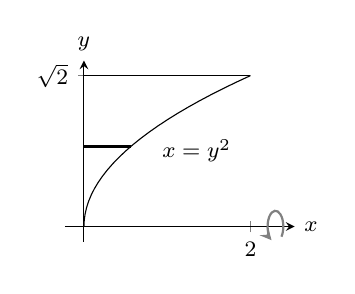
\begin{tikzpicture}[font=\footnotesize,declare function={f(\x)=\x^2;}]
\pgfmathsetmacro{\c}{0.75}
\begin{axis}[clip=false,width=4.5cm,axis lines=middle,xlabel={$x$},ylabel={$y$},xlabel style={at={(current axis.right of origin)},anchor=west},ylabel style={at={(current axis.above origin)},anchor=south},xtick={2},ytick={1.4142}, yticklabels={$\sqrt{2}$},enlargelimits=true,ymin=0,xmax=2.3]
\addplot[domain=0:sqrt(2)]({f(x)},{x})node[pos=0.5,below right]{$x=y^2$};
\draw[gray,thick,-stealth]([shift={(-40:0.1cm and 0.2cm)}]2.3,0) arc (-40:240:0.1cm and 0.2cm);
\draw[thick](axis cs:{f(\c)},\c)--(axis cs:0,\c);
\draw[](axis cs:{f(sqrt(2))},{sqrt(2)})--(axis cs:0,{sqrt(2)});
\end{axis}
\end{tikzpicture}
\caption{}
\label{شکل_سوال_تکمل_استعمال_ترکیب_چھلا_پ}
\end{minipage}
\end{figure}
%
\begin{figure}
\centering
\begin{minipage}{0.3\textwidth}
\centering
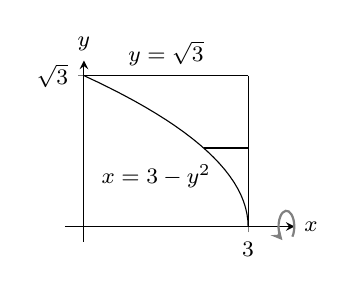
\begin{tikzpicture}[font=\footnotesize,declare function={f(\x)=3-\x^2;}]
\pgfmathsetmacro{\c}{0.9}
\pgfmathsetmacro{\ky}{sqrt(3)}
\begin{axis}[clip=false,width=4.5cm,axis lines=middle,xlabel={$x$},ylabel={$y$},xlabel style={at={(current axis.right of origin)},anchor=west},ylabel style={at={(current axis.above origin)},anchor=south},xtick={3},ytick={\ky}, yticklabels={$\sqrt{3}$},enlargelimits=true,xmax=3.5]
\addplot[domain=0:sqrt(3)]({f(x)},{x})node[pos=0.25,left,yshift=-1ex,font=\footnotesize]{$x=3-y^2$};
\draw[gray,thick,-stealth]([shift={(-40:0.1cm and 0.2cm)}]3.7,0) arc (-40:240:0.1cm and 0.2cm);
\draw[thick](axis cs:{f(\c)},\c)--(axis cs:3,\c);
\draw[](axis cs:0,{sqrt(3)})--(axis cs:3,{sqrt(3)})node[pos=0.5,above]{$y=\sqrt{3}$};
\draw(3,{sqrt(3)})--(3,0);
\end{axis}
\end{tikzpicture}
\caption{}
\label{شکل_سوال_تکمل_استعمال_ترکیب_چھلا_ت}
\end{minipage}\hfill
\begin{minipage}{0.3\textwidth}
\centering
\begin{tikzpicture}[font=\footnotesize,declare function={f(\x)=sqrt(\x^2+1);}]
\pgfmathsetmacro{\k}{sqrt(3)}
\begin{axis}[clip=false,width=4.5cm,axis lines=middle,xlabel={$x$},ylabel={$y$},xlabel style={at={(current axis.right of origin)},anchor=west},ylabel style={at={(current axis.above origin)},anchor=south},xtick={\k},xticklabels={$\sqrt{3}$}, ytick={1,2},enlargelimits=true,ymin=0]
\addplot[domain=0:\k]{f(x)}node[pos=0.75,above left]{$y=\sqrt{x^2+1}$};
\draw(axis cs:\k,{f(\k)})--(axis cs:\k,0)node[pos=0.5,right]{$x=\sqrt{3}$};
\draw({1/2*sqrt(3)},0.5)node[]{\RL{$y$ محور}};
\end{axis}
\end{tikzpicture}
\caption{}
\label{شکل_سوال_تکمل_استعمال_ترکیب_چھلا_ٹ}
\end{minipage}\hfill
\begin{minipage}{0.3\textwidth}
\centering
\begin{tikzpicture}[font=\footnotesize,declare function={f(\x)=9*\x/sqrt(\x^3+9);}]
\begin{axis}[clip=false,width=4.5cm,axis lines=middle,xlabel={$x$},ylabel={$y$},xlabel style={at={(current axis.right of origin)},anchor=west},ylabel style={at={(current axis.above origin)},anchor=south},xtick={3}, ytick={5},ymax=5.5,enlargelimits=true,ymin=0]
\addplot[domain=0:3]{f(x)}node[pos=0.95,above left]{$y=\tfrac{9x}{\sqrt{x^3+9}}$};
\draw(axis cs:3,{f(3)})--(axis cs:3,0);
\draw(1.5,1.5)node[above]{\RL{$y$ محور}};
\end{axis}
\end{tikzpicture}
\caption{}
\label{شکل_سوال_تکمل_استعمال_ترکیب_چھلا_ث}
\end{minipage}
\end{figure}

سوال \حوالہ{سوال_تکمل_استعمال_ترکیب_خول_سے_تلاش_الف} تا سوال \حوالہ{سوال_تکمل_استعمال_ترکیب_خول_سے_تلاش_ب} میں دیے منحنیات اور لکیروں میں محیط خطے کو \عددی{y} محور کے گرد گھما کر جسم طواف پیدا کیا جاتا ہے۔ اس جسم کا حجم ترکیب خول سے تلاش کریں۔

\ابتدا{سوال}\شناخت{سوال_تکمل_استعمال_ترکیب_خول_سے_تلاش_الف}
$y=x,\quad y=-\tfrac{x}{2},\quad x=2$
\انتہا{سوال}
%=====================
\ابتدا{سوال}
$y=2x,\quad y=\tfrac{x}{2},\quad x=1$
\انتہا{سوال}
%=====================
\ابتدا{سوال}
$y=x^2,\quad y=2-x,\quad x=0, (x\ge 0)$
\انتہا{سوال}
%=====================
\ابتدا{سوال}
$y=2-x^2,\quad y=x^2,\quad x=0$
\انتہا{سوال}
%=====================
\ابتدا{سوال}
$y=\sqrt{x},\quad y=0,\quad x=4$
\انتہا{سوال}
%=====================
\ابتدا{سوال}
$y=2x-1,\quad y=\sqrt{x},\quad x=0$
\انتہا{سوال}
%=====================
\ابتدا{سوال}
$y=\tfrac{1}{x},\quad y=0,\quad x=\tfrac{1}{2},\quad x=2$
\انتہا{سوال}
%=====================
\ابتدا{سوال}\شناخت{سوال_تکمل_استعمال_ترکیب_خول_سے_تلاش_ب}
$y=\tfrac{3}{2\sqrt{x}},\quad y=0,\quad x=1,\quad x=4$
\انتہا{سوال}
%=====================
سوال \حوالہ{سوال_تکمل_استعمال_محور_طواف_وائے_الف} تا سوال \حوالہ{سوال_تکمل_استعمال_محور_طواف_وائے_ب} میں طواف جسم کا حجم ترکیب خول سے معلوم کریں۔ منحنیات اور لکیروں میں محیط رقبہ کو \عددی{y} محور کے گرد گھمایا گیا ہے۔

\ابتدا{سوال}\شناخت{سوال_تکمل_استعمال_محور_طواف_وائے_الف}
$x=\sqrt{y},\quad x=-y,\quad y=2$
\انتہا{سوال}
%=========================
\ابتدا{سوال}
$x=y^2,\quad x=-y,\quad y=2$
\انتہا{سوال}
%=========================
\ابتدا{سوال}
$x=2y-y^2,\quad x=0$
\انتہا{سوال}
%=========================
\ابتدا{سوال}
$x=2y-y^2,\quad x=y$
\انتہا{سوال}
%=========================
\ابتدا{سوال}
$y=\abs{x},\quad y=1$
\انتہا{سوال}
%=========================
\ابتدا{سوال}
$y=x,\quad y=2x,\quad y=2$
\انتہا{سوال}
%=========================
\ابتدا{سوال}
$y=\sqrt{x},\quad y=0,\quad y=x-2$
\انتہا{سوال}
%=========================
\ابتدا{سوال}\شناخت{سوال_تکمل_استعمال_محور_طواف_وائے_ب}
$y=\sqrt{x},\quad y=0,\quad y=2-x$
\انتہا{سوال}
%=========================

سوال \حوالہ{سوال_تکمل_استعمال_کئی_محور_الف} اور سوال \حوالہ{سوال_تکمل_استعمال_کئی_محور_ب} میں سایہ دار خطے کو  دیے گئے محور کے گرد گھما کر جسم طواف پیدا کیا جاتا ہے۔ اس جسم کا حجم ترکیب خول سے معلوم کریں۔ 

\ابتدا{سوال}\شناخت{سوال_تکمل_استعمال_کئی_محور_الف}
خطے کو شکل \حوالہ{شکل_سوال_تکمل_استعمال_کئی_محور_الف} میں دکھایا گیا ہے۔
\begin{enumerate}[a.]
\item
محور \عددی{x} کے گرد،
\item
محور طواف لکیر \عددی{y=1} ہے،
\item
محور طواف لکیر \عددی{y=\tfrac{8}{5}} ہے،
\item
لکیر \عددی{y=-\tfrac{2}{5}} کے گرد گھمایا جاتا ہے۔
\end{enumerate}
\انتہا{سوال}
%====================
\ابتدا{سوال}\شناخت{سوال_تکمل_استعمال_کئی_محور_ب}
خطے کو شکل \حوالہ{شکل_سوال_تکمل_استعمال_کئی_محور_ب} میں دکھایا گیا ہے۔
\begin{enumerate}[a.]
\item
محور \عددی{x} کے گرد،
\item
محور طواف لکیر \عددی{y=2} ہے،
\item
محور طواف لکیر \عددی{y=5} ہے،
\item
لکیر \عددی{y=-\tfrac{5}{8}} کے گرد گھمایا جاتا ہے۔
\end{enumerate}
\انتہا{سوال}
%====================
\begin{figure}
\centering
\begin{minipage}{0.45\textwidth}
\centering
\begin{tikzpicture}[font=\footnotesize,declare function={f(\x)=12*(\x^2-\x^3);}]
\begin{axis}[axis on top,clip=false,width=4.5cm,axis lines=middle,xlabel={$x$},ylabel={$y$},xlabel style={at={(current axis.right of origin)},anchor=west},ylabel style={at={(current axis.above origin)},anchor=south},xtick={1},ytick={1},enlargelimits=true]
\addplot[domain=-0.2:1]({f(x)},x)node[pos=0.75,above]{$x=12(y^2-y^3)$};
\addplot[name path=fun,domain=0:1,draw=none]({f(x)},x);
\draw[name path=axis](0,0)--(0,1);
\addplot[fill=lgray]fill between[of=fun and axis];
\end{axis}
\end{tikzpicture}
\caption{}
\label{شکل_سوال_تکمل_استعمال_کئی_محور_الف}
\end{minipage}\hfill
\begin{minipage}{0.45\textwidth}
\centering
\begin{tikzpicture}[font=\footnotesize,declare function={f(\x)=1/4*\x^4-1/2*\x^2;g(\x)=1/2*\x^2;}]
\begin{axis}[axis on top,clip=false,width=4.5cm,axis lines=middle,xlabel={$x$},ylabel={$y$},xlabel style={at={(current axis.right of origin)},anchor=west},ylabel style={at={(current axis.above origin)},anchor=south},xtick={1,2},ytick={2},enlargelimits=true]
\addplot[name path=funf,domain=0:2]({f(x)},x)node[pos=0.75,above,yshift=0.5ex]{$x=\tfrac{y^4}{4}-\tfrac{y^2}{2}$};
\addplot[name path=fung,domain=0:2]({g(x)},x)node[pos=0.5,right]{$x=\tfrac{y^2}{2}$};
\draw[name path=axis](2,0)--(2,2);
\addplot[fill=lgray]fill between[of=funf and axis];
\addplot[fill=white]fill between[of=fung and axis];
\end{axis}
\end{tikzpicture}
\caption{}
\label{شکل_سوال_تکمل_استعمال_کئی_محور_ب}
\end{minipage}
\end{figure}

سوال \حوالہ{سوال_تکمل_استعمال_چھلا_خول_الف} تا سوال \حوالہ{سوال_تکمل_استعمال_چھلا_خول_الف} میں خطوں کو محور طواف کے گرد گھما کر حاصل جسم طواف کا حجم معلوم کریں۔ آپ ترکیب چھلا یا ترکیب خول استعمال کر سکتے ہیں۔

\ابتدا{سوال}\شناخت{سوال_تکمل_استعمال_چھلا_خول_الف}
تکون جس کے راس \عددی{(1,1)}، \عددی{(1,2)} اور \عددی{(2,2)} ہیں۔ (ا) \عددی{x} محور کے گرد، (ب) \عددی{y} محور کے گرد، (ج) لکیر \عددی{x=\tfrac{10}{3}} کے گرد، اور (د) لکیر \عددی{y=1} کے گرد۔
\انتہا{سوال}
%=======================
\ابتدا{سوال}
ربع اول میں منحنی \عددی{x=y-y^3} اور \عددی{y} محور میں محیط خطہ کو (ا) محور \عددی{x}، (ب) لکیر \عددی{y=1} کے گرد گھمایا جاتا ہے 
\انتہا{سوال}
%======================
\ابتدا{سوال}
ربع اول میں \عددی{x=y-y^3}، \عددی{x=1} اور \عددی{y=1} میں محیط خطہ کو (ا) محور \عددی{x}، (ب) محور \عددی{y}، (ج) لکیر \عددی{x=1}، اور (د) لکیر \عددی{y=1} کے گرد گھمایا جاتا ہے۔
\انتہا{سوال}
%=============================
\ابتدا{سوال}
تکونی خطہ جس کے سرحد لکیر \عددی{2y=x+4}، \عددی{y=x}، اور \عددی{x=0} ہیں کو (ا) محور \عددی{x}، (ب) محور \عددی{y}، (ج) لکیر \عددی{x=4}، اور (د) لکیر \عددی{y=8} کے گرد گھمایا جاتا ہے۔
\انتہا{سوال}
%=====================
\ابتدا{سوال}
ربع اول میں \عددی{y=x^3}، \عددی{y=4x} کے بیچ خطہ کو (ا) محور \عددی{x}، اور (ب) لکیر \عددی{y=8} کے گرد گھمایا جاتا ہے۔
\انتہا{سوال}
%=========================
\ابتدا{سوال}
سرحد \عددی{y=\sqrt{x}} اور \عددی{y=\tfrac{x^2}{8}} میں محیط خطہ کو (ا) محور \عددی{x} اور (ب) محور \عددی{y} کے گرد گھمایا جاتا ہے۔
\انتہا{سوال}
%=======================
\ابتدا{سوال}
سرحد \عددی{y=2x-x^2} اور \عددی{y=x} میں محیط خطہ کو (ا) محور \عددی{y} اور (ب) لکیر \عددی{x=1} کے گرد گھمایا جاتا ہے۔
\انتہا{سوال}
%========================
